\section{Durchführung}
\label{sec:Durchführung}
Zur Bestimmung der Molwärme wird in diesem Versuch ein Kupferzylinder mithilfe 
von flüssigem Stickstoff stark abgekühlt und anschließendn mit einem Heizstrom erhitzt. 
Die zugefügt Wärmeenergie und die Temperaturänderung werden jeweils gemessen, 
woraus dann die Molwärme berechnet werden kann. 
\\

Dafür wird ein Aufbau wie in Abbildung \ref{fig:aufbau} verwendet. 
In ein Dewar-Gefäß, in dem später flüssiger Stickstoff eingefüllt wird,
wird ein Zylinder gehängt, um den eine Heizdraht gewickelt ist. 
Darin befindet sich die Kupferrobe mit einem weiteren Heizdraht. 
Der Zylinder ist an eine Vakuumpumpe und an eine Heliumflasche angeschlossen, wobei diese 
getrennt voneinander mit einem Absperrhahn %
Die Heizdrähte sind jeweils mit einer Heizspannung, einem Voltmeter und einem Amperemeter
verbunden. Die Temperaturänderung der Probe sowie die Temperatur des Zylinders wird jeweils mit einem Ohmmeter ermittelt.
\FloatBarrier
\begin{figure}
  \centering
  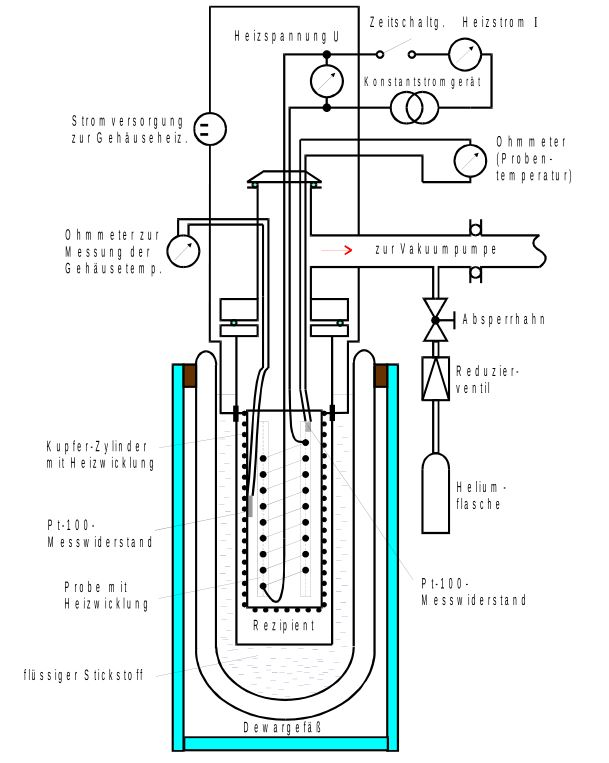
\includegraphics[width=0.55\textwidth]{Aufbau.JPG}
  \caption{Versuchsaufbau [1].}
  \label{fig:hkurve}
\end{figure}
\FloatBarrier

Zunächst muss die Probe soweit es geht runtergekühlt werden. Dafür wird der Zylinder mithilfe der Vakuumpumpe evakuiert und dann 
mit Helium gefüllt. Anschließend wird das Dewar-Gefäß mit Flüssigstickstoff gefüllt. Das Helium erhöht die Wärmeleitfähigkeit 
zwischen Zylinder und Probe. Nun wird so lange gewartet, bis die Temperatur der Probe nicht mehr weiter sinkt, 
was nach ungefähr einer Stunde und einer Temperatur von $\SI{190}{\celsius}$ eintritt. 
Der am Ohmmeter angezeigte Widerstand $R$ kann dabei mit einer Tabelle oder der Formel 
\begin{equation}
    \label{eqn:T}
    T = 0,00134 R^2 + 2,296 R -243,02
\end{equation}
in die Temperatur $T$ umgerechnet werden.
\\

Danach wird das Helium mit der Vakuumpumpe wieder aus dem Zylinder gepumpt. Es wird nun das Heizstromgerät für 
die Probe eingeschaltet und gleichzeitig eine Stoppuhr gestartet. Dabei wird die Spannung sowie der Strom notiert. 
Sobald die Probe um eine Temperatur von etwa $\SI{7}{\celsius}-\SI{11}{\celsius}$
gestiegen ist, wird der Heizstrom ausgestellt und die Zeit gestoppt. Die Zeit wird ebenfalls notiert. 
Das wird dann so lange wiederholt, bis die Probe eine Temperatur von etwa $\SI{30}{\celsius}$ 
erreicht hat. 

Während der gesamten Messung muss der Zylinder die gleiche Temperatur wie die Probe haben, damit 
diese keine Wärme vom Zylinder aufnimmt oder Wärme an ihn abgibt, da das die Messwerte verfälschen würde. 
Dafür wird bei dem zweiten Heizstromgerät der Strom und die Spannung so eingestellt, dass der Zylinder eine ähnliche Temperatur wie die Probe hat. 